\documentclass[aspectratio=169]{beamer}
\usepackage{braket,caption}
\usetheme{focus}
\newcommand{\focus}[1]{\textcolor{blue}{\textbf{#1}}}
\newcommand{\cen}[1]{\begin{center}{#1}\end{center}}

\definecolor{main}{RGB}{40, 40, 40}

\title{
\vspace*{\fill}
\LARGE{Journey from the Hubbard Dimer\\
to the Hubbard Model}
\vspace*{\fill}
}
\vspace*{\fill}
\author{Abhirup Mukherjee, Dr. Siddhartha Lal}
\vspace*{\fill}
\institute{Department of Physical Sciences\\IISER Kolkata}
\vspace*{\fill}
\date{\today}
\vspace*{\fill}
\begin{document}
\begin{frame}{}
\maketitle
\end{frame}

\begin{frame}{Overview of the Process}
\begin{itemize}[<alert@+>]
	\item Choose correlated Anderson model as the auxiliary model and perform URG analysis and extract zero mode to obtain Hubbard dimer as the effective low energy Hamiltonian.
	\item Translate this Hubbard dimer Hamiltonian to recreate a new/renormalized Hubbard model. This Hubbard model is assumed to be linked to the parent Hubbard model via a similarity transformation.
	\item Express equation between renormalized Hubbard and Hubbard dimers as relation between inverse Greens function matrix elements of full Hubbard model and those of the Hubbard dimer.
	\item Obtain Greens functions of the parent Hubbard model in terms of those of the Hubbard dimer.
\end{itemize}
\end{frame}

\begin{frame}{Cluster-Bath Approach}
	\begin{figure}[htpb]
		\centering
		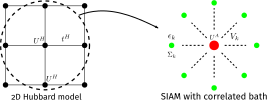
\includegraphics[width=0.6\textwidth]{./cluster-bath.png}
	\end{figure}

\begin{minipage}{0.49\textwidth}
\begin{equation*}
-t^H\sum_{\sigma,\left<i,j \right>}\left(c^\dagger_{i\sigma} c_{j\sigma} + \text{h.c.}\right) + U^H\sum_i \tau_{i \uparrow} \tau_{i \downarrow}
\end{equation*}
\end{minipage}
\begin{minipage}{0.49\textwidth}
	\begin{equation*}\begin{aligned}
\sum_{k\sigma}\tilde\epsilon_k\tau_{k\sigma} + U^A \tau_{d \uparrow} \tau_{d \downarrow} + U_b \sum_{kk^\prime}\hat n_k \hat n_{k^\prime}\\
-t^A\sum_{k\sigma}\left(c^\dagger_{d\sigma}c_{k\sigma} + \text{h.c.}\right)
\end{aligned}\end{equation*}
\end{minipage}
\end{frame}
\begin{frame}{RG Analysis of Auxiliary System}
	\[\sum_{k\sigma}\tilde\epsilon_k\tau_{k\sigma} + U \tau_{d \uparrow} \tau_{d \downarrow} + U_b \sum_{kk^\prime}\hat n_k \hat n_{k^\prime} -t\sum_{k\sigma}\left(c^\dagger_{d\sigma}c_{k\sigma} + \text{h.c.}\right)\]
	\[\Bigg\downarrow U H U^\dagger\]
	\[\sum_{k\sigma}^*\left[\tilde\epsilon_k\tau_{k\sigma} -{t}^*\left(c^\dagger_{d\sigma}c_{k\sigma} + \text{h.c.}\right)\right] + U^* \tau_{d \uparrow} \tau_{d \downarrow} + U^* \sum_{kk^\prime}^*\hat n_k \hat n_{k^\prime} \]
	\[\Bigg\downarrow \text{zero mode}\]
	\[-{t}^*\sum_{\sigma}^*\left(c^\dagger_{d\sigma}c_{z\sigma} + \text{h.c.}\right) + U^* \tau_{d \uparrow} \tau_{d \downarrow} + U^* \tau_{z \uparrow} \tau_{z \downarrow} \]
\end{frame}
\begin{frame}{RG Analysis of Auxiliary System}
	\only<+>{
\cen{\focus{Lattice of \(N\) sites and \(Z\) nearest neighburs at each site}}
\begin{equation*}
	H = -t^H \sum_{\left<ij\right>}\left(c^\dagger_{i\sigma}c_{j\sigma} + \text{h.c.}\right) + \sum_i U^H \hat n_{i \uparrow} \hat n_{i \downarrow} - \mu^H \hat N
\end{equation*}
\begin{itemize}
	\item For particle-hole symmetry, choose \(U^H = \frac{1}{2}\mu^H\)
	\item Define \(\tau = \hat n - \frac{1}{2}\).
\end{itemize}
{\Large
\begin{equation*}\begin{aligned}
	H = -t^H \sum_{\left<ij\right>}\left(c^\dagger_{i\sigma}c_{j\sigma} + \text{h.c.}\right) + \sum_i U^H\tau_{i \uparrow}\tau_{i \downarrow}
\end{aligned}\end{equation*}
}
}
\only<+>{
	\begin{itemize}
		\item Express entire thing in terms of nearest-neighbour pairs
\begin{equation*}\begin{aligned}
	  &= -t^H \sum_{\left<ij\right>}\left(c^\dagger_{i\sigma}c_{j\sigma} + \text{h.c.}\right) + \frac{1}{Z}\sum_{\left<ij\right>} U^H\left[\tau_{i \uparrow}\tau_{i \downarrow} + \tau_{j \uparrow}\tau_{j \downarrow}\right]\\
	  &= \frac{1}{Z}\sum_{\left<ij\right>}\left[-Zt^H \left(c^\dagger_{i\sigma}c_{j\sigma} + \text{h.c.}\right) +  U^H\left(\tau_{i \uparrow}\tau_{i \downarrow} + \tau_{j \uparrow}\tau_{j \downarrow}\right)\right]\\
\end{aligned}\end{equation*}
\item Since total number of nearest neighbours pairs is \(\frac{NZ}{2}\), pull out the same factor
\begin{equation}\begin{aligned}
	H &= \frac{2}{NZ}\sum_{\left<ij\right>}\left[-\frac{NZt^H}{2} \left(c^\dagger_{i\sigma}c_{j\sigma} + \text{h.c.}\right) +  \frac{NU^H}{2}\left(\tau_{i \uparrow}\tau_{i \downarrow} + \tau_{j \uparrow}\tau_{j \downarrow}\right)\right]\\
\end{aligned}\end{equation}
\end{itemize}
}
\only<+>{
	\cen{\focus{The final Hamiltonian is a sum of Hubbard dimers}}
\begin{equation*}
	H = \frac{2}{NZ}\sum_{\left<ij \right>}H^D\left(i, j, t^D = \frac{NZt^H}{2}, U^D = \frac{NU^H}{2}\right)
\end{equation*}
\centering
	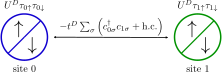
\includegraphics[width=0.55\textwidth]{./hubb_dim.png}
\vspace*{\fill}
	\Large
	\begin{equation*}\begin{aligned}
		H^D = -t^D\left(c^\dagger_{0\sigma}c_{1\sigma} + \text{h.c.}\right) + U^D\left(\tau_{0 \uparrow}\tau_{0 \downarrow} + \tau_{1 \uparrow}\tau_{1 \downarrow}\right)
	\end{aligned}\end{equation*}
}
\end{frame}

\begin{frame}{Inverse Greens function from Hamiltonian}
	\cen{\focus{Write equation in terms of inverse Greens function \(G^{-1}(\omega) = \omega - H\)}}
	\begin{equation*}\begin{aligned}
		\omega - G^{-1} &= \frac{2}{NZ}\sum_{\left<ij \right>}\left[\omega - G^{-1}_D(\omega, i, j)\right]\\
	\longrightarrow G^{-1} &= \frac{2}{NZ}\sum_{\left<ij \right>}G^{-1}_D(\omega, i, j)
\end{aligned}\end{equation*}
\begin{itemize}
	\only<+>{
		\item Take diagonal matrix element \(\bra{i}G^{-1}\ket{i}\). On the RHS, there are \(Z\) terms that have the index \(i\). Because of translational invariance, all such terms will be same.
	\begin{equation*}
		\left(G^{-1}\right)_{ii} = \frac{2}{NZ}\times \left(G_D^{-1}\right)_{ii}\times Z = \frac{2}{N}\left(G_D^{-1}\right)_{00}
	\end{equation*}
}
\only<+>{
\item Take nearest-neighbour matrix element \(\bra{i}G^{-1}\ket{j}\). On the RHS, there's just one term that has both indices \(i\) and \(j\).
	\begin{equation*}
		\left(G^{-1}\right)_{ij} = \frac{2}{NZ}\times \left(G_D^{-1}\right)_{ij} = \frac{2}{NZ}\left(G_D^{-1}\right)_{01} 
	\end{equation*}
}
\only<+>{
\item \focus{All other matrix elements are zero}, because no term in the Hamiltonian scatters between non-nearest-neighbour sites \\
	\(\longrightarrow\) \focus{tri-diagonal inverse Greens function matrix}
}
\end{itemize}
\end{frame}

\begin{frame}{Diagonalizing the inverse Greens function matrix}
	\only<+>{
	\begin{equation*}
		G^{-1} = \begin{pmatrix} g_0 & g_1 & ... & ... & g_1 \\
			g_1 & g_0 & g_1 & ... & ... \\
			    & g_1 & g_0 & g_1 & ...\\
			    && ... &&
	\end{pmatrix} 
	\xrightarrow{\text{Fourier transform to $k-$space}}
			g_0 + g_1\begin{pmatrix} \xi_{\vec k_1} &&&...\\
				& \xi_{\vec k_2} &&...\\ 
				&& \xi_{\vec k_3} &...\\
				&...&&
	\end{pmatrix}
\end{equation*}
\begin{equation*}
	\xi_{\vec k} = \sum_\text{i=1}^Z \cos (a_i q_i)
\end{equation*}
}
\only<2>{
{\large
\begin{equation*}
	G^{-1} = g_0 + g_1\begin{pmatrix} \xi_{\vec k_1} &&&...\\
				& \xi_{\vec k_2} &&...\\ 
				&& \xi_{\vec k_3} &...\\
				&...&&
	\end{pmatrix}
		\xrightarrow{\text{invert the diagonal matrix}}
		G = \begin{pmatrix} G_{\vec k_1} &&&...\\
				& G_{\vec k_2} &&...\\ 
				&& G_{\vec k_3} &...\\
				&...&&  \end{pmatrix} 
\end{equation*}
}
}
\end{frame}
\begin{frame}{Compute Greens functions and other stuff}
\large
\begin{equation*}\begin{aligned}
	\only<1-4>{
	\text{\focus{$\color{blue}{\vec k}$-space Greens function: }}\quad G_H (\vec k, \omega) &= \frac{N}{2}\left\{\left[G_{D}^{-1}(\omega)\right]_{00} + \frac{1}{Z}\left[G_{D}^{-1}(\omega)\right]_{01}\xi_{\vec k}\right\}^{-1}\\[20pt]}
	\only<2-4>{
	\text{$\color{blue}{\vec r}$\focus{-space Greens function: }}\quad G_H (\vec r, \omega) &= \frac{1}{2}\sum_{\vec k}\left\{\left[G_{D}^{-1}(\omega)\right]_{00} + \frac{1}{Z}\left[G_{D}^{-1}(\omega)\right]_{01}\xi_{\vec k}\right\}^{-1}\\[20pt]}
	\only<3-4>{
	\text{\focus{self-energy: }}\quad \Sigma_H (\vec k, \omega) &= \omega - g_0 + \left(t^H - g_1\right)\xi_{\vec k}\\[20pt]}
\end{aligned}\end{equation*}
\only<4-4>{
	\centering
	\focus{Greens functions give spectral functions as well!}
}
\end{frame}

\begin{frame}{On the Bethe Lattice $(Z \to \infty)$}
\begin{minipage}{0.59\textwidth}
\centering
\only<+>{
Hamiltonian scaling arguments suggest \footnotemark
\begin{equation*}
	G_{ij} \sim G_{ii}\delta_{ij}
\end{equation*}
(\focus{Greens function becomes local})
}
\only<+>{
Also emerges from this formulation:

\begin{equation*}
G^{-1}_{ii} = \frac{2}{N}\left[G^{-1}_D\right]_{00} \to \text{finite}
\end{equation*}
\begin{equation*}
	\mathbf{\textcolor{blue}{G^{-1}_{ij} = \frac{2}{NZ}\left[G^{-1}_D\right]_{00} \to 0}} \quad\text{ when } Z \to \infty
\end{equation*}
\\[20pt]


\(G^{-1}_{ij}\) becomes diagonal
\(\longrightarrow \color{blue}{G_{ij}} \) \focus{becomes diagonal}
}
\end{minipage}
\begin{minipage}{0.4\textwidth}
	\centering
	\includegraphics[width=0.7\textwidth]{./bethe.png}\\[20pt]
	Bethe lattice with \(Z=3\)
\end{minipage}
\footnotetext{Vollhardt, Krzysztof and Marcus, Dynamical Mean-Field Theory, 2012, Springer Berlin Heidelberg}
\end{frame}

\end{document}
